\documentclass[12pt]{article}

\usepackage{amsmath, amsthm, amssymb}
\usepackage{enumitem}
\usepackage[margin=2.5cm]{geometry}
\usepackage{setspace}
\usepackage{graphicx}
\graphicspath{ {./images/} }

\renewcommand{\baselinestretch}{1.5}
\everymath{\displaystyle}

\begin{document}
	\section*{Q1}
	\begin{enumerate}[label=\alph*)]
		\item $\mathbb{E}[\mathcal{L}(y=\text{Keep},t)]=0.1\times 1=0.1$\\
		$\mathbb{E}[\mathcal{L}(y=\text{Remove},t)]=0.9\times 100=90$
		\item We want to minimize expected loss given conditional probability, let $p=Pr(t=\text{Spam}|x)$, so compute $\min\mathbb{E}[\mathcal{L}(y=\text{Keep},t)]\cdot Pr(t=\text{Spam}|x)=p$ and $\min\mathbb{E}[\mathcal{L}(y=\text{Remove},t)]\cdot Pr(t=\text{Not Spam}|x)=100(1-p)$.\\
		Set $p=100(1-p)$, calculate to get $p=\frac{100}{101}$, so if $Pr(t=\text{Spam}|x)\leq\frac{100}{101}$, keep the email, if $Pr(t=\text{Spam}|x)>\frac{100}{101}$, remove the email.
		\item We can use conditional probability formula to compute $Pr(Spam|x)$, i.e. $Pr(Spam|x)=\frac{Pr(x|Spam)Pr(Spam)}{Pr(x)}$.\\
		$Pr(Spam|x=(0,0))=\frac{0.4\times0.1}{0.4\times0.1+0.998\times0.9}=0.043$\\
		$Pr(Spam|x=(0,1))=\frac{0.3\times0.1}{0.3\times0.1+0.001\times0.9}=0.971$\\
		$Pr(Spam|x=(1,0))=\frac{0.1\times0.1}{0.1\times0.1+0\times0.9}=0.957$\\
		$Pr(Spam|x=(1,1))=\frac{0.1\times0.1}{0.1\times0.1+0\times0.9}=1$\\
		From what we have in b), if $x=(1,1)$, remove the email, otherwise if $x=(0,0),(0,1)\;or\;(1,0)$, keep the email
	\end{enumerate}
		
	\newpage
	
	\section*{Q2}
	\begin{enumerate} [label=\alph*)]
		\item The three points are on the same line, so they can't be in two different half-space at the same time, so this dataset is not linearly separable.
		\item \begin{tabular}{c|c|c}
			$\psi_1(x)$ & $\psi_2(x)$ & t \\
			\hline
			-1 & 1 & 1 \\
			1 & 1 & 0 \\
			3 & 9 & 1 \\
		\end{tabular} \\
		We want $w^\top x\geq0$ when $t=1$, $w^\top x<0$ when $t=0$, so \[-w_1+w_2\geq0\quad w_1+w_2<0\quad3w_1+9w_2\geq0\]
		From the inequalities above, $(-2,1)$ correctly classify all the examples
	\end{enumerate}
	\newpage
	
	\section*{Q3}
	\subsection*{3.1}
	\begin{enumerate}[label=\alph*)]
		\item 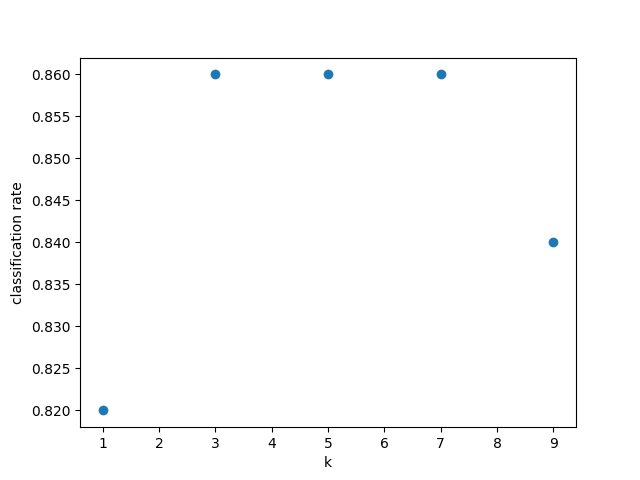
\includegraphics[scale=0.6]{3.1a.png}
		\item Choose $k=5$ because when $k=5$ the highest accuracy of $86\%$ is achieved. The accuracy also have a trend to first increase then decrease, so choose $5$ instead of $3$ and $7$ because $5$ is in the middle, and more likely to have high accuracy with different dataset.\\
		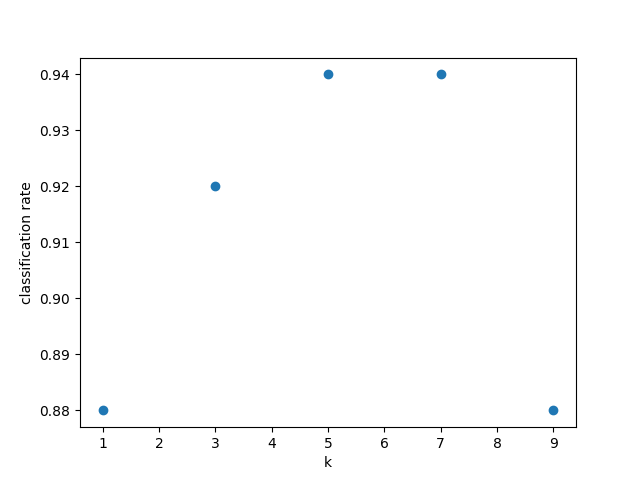
\includegraphics[scale=0.6]{3.1b.png}\\
		Classification rate for $k^*=5$ is $94\%$, $k^*-2=3$ have accuracy $92\%$, $k^*+2=7$ have accuracy $94\%$, the accuracy of test data is higher than that of validation data for all values of $k$.
	\end{enumerate}
	\subsection*{3.2}
	\begin{enumerate}[label=\alph*)]
		\item see python file
		\item For mnist\_train, use learning rate $0.2$ and iterations $800$ as hyperparameters, these are the parameters that yield a small entropy and high classification; for training data, final cross entropy is $0.014$ and classification rate is $100\%$, for validation data, final cross entropy is $0.192$, the classification is $88\%$, for test data, final cross entropy is $0.227$, the classification is $92\%$.\\
		For mnist\_train\_small, use learning rate $0.4$ and iterations $1000$ as hyperparameters, they generate relatively low entropy and high classification rate;  for training data, final cross entropy is $0.0006$ and classification rate is $100\%$, for validation data, final cross entropy is $0.954$, the classification is $74\%$, for test data, final cross entropy is $0.966$, the classification is $78\%$.
		\item The plot are as followed. The results change due to change in initial weights and bias when using random weights. In this case, try several times and take an average over a set of entropy values of classification rates, then decide the best hyperparameters choice.\\ 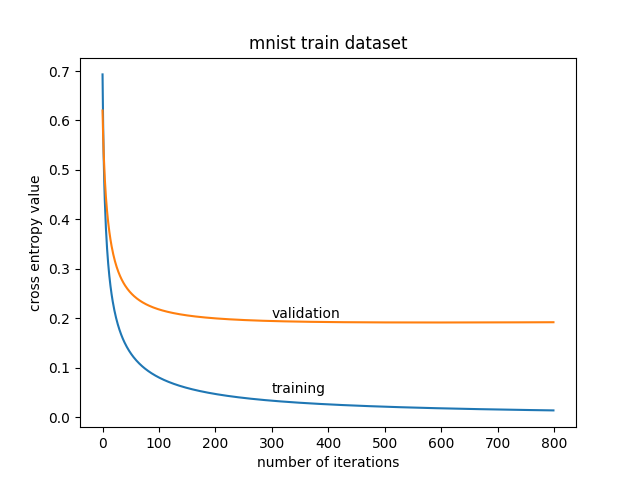
\includegraphics[scale=0.5]{3.2c1.png}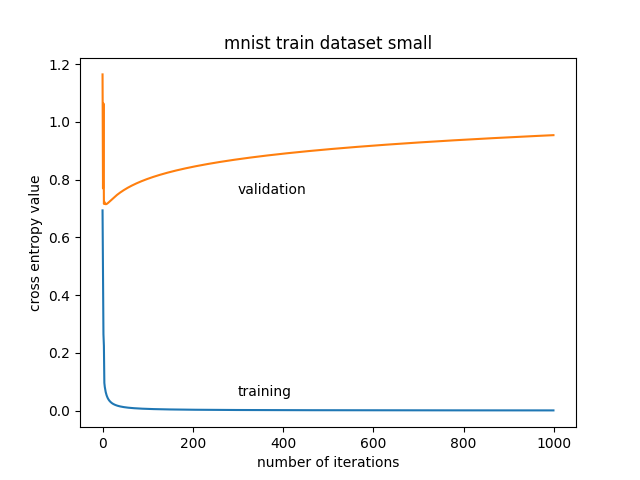
\includegraphics[scale=0.5]{3.2c2.png}
		
	\end{enumerate}
	\newpage
	
	\section*{Q4}
	\begin{enumerate}[label=\alph*)]
		\item Note the function is sum of squares, so it's sum of convex functions, so it's convex and the local minimum (obtained when gradient to 0) is the global minimum. The design matrix $X$ is the matrix with $x(i)$ on row $i$, and let $y$ be the vector with $y(i)$ on row $i$, so this problem can be re-write as:
		\begin{align*}
			f(w) &= \frac{1}{2}(y-Xw)^TA(y-Xw)+\frac{\lambda}{2}||w||^2\\
			&=\frac{1}{2}(y^T-w^TX^T)A(y-Xw)+\frac{\lambda}{2}||w||^2\\
			&=\frac{1}{2}(y^TAy-y^TAXw-w^TX^TAy+w^TX^TAXw)+\frac{\lambda}{2}||w||^2I
		\end{align*}
		Differentiate with respect to $w$:
		\[\triangledown f=\frac{1}{2}(-y^TAX-y^TAX+2X^TAXw)+\lambda wI\]
		Set to $0$ to find minimum point:
		\begin{align*} &\frac{1}{2}(-y^TAX-y^TAX+2X^TAXw)+\lambda wI=0\\
			&X^TAXw+\lambda wI=y^TAX\\
			&w=(X^TAX+\lambda I)^{-1}X^TAy
		\end{align*}
	as desired.
		\item Sorry I can't figure out how to use the l2 function
		
	\end{enumerate}
	
	
	
	
	
	
	
\end{document}